% *********************************************************************
% © 2016–2026 Jeremy Sylvestre
%
% Permission is granted to copy, distribute and/or modify this document
% under the terms of the GNU Free Documentation License, Version 1.3 or
% any later version published by the Free Software Foundation; with no
% Invariant Sections, no Front-Cover Texts, and no Back-Cover Texts. A
% copy of the license is included in the appendix entitled “GNU Free
% Documentation License” that appears in the output document of this
% PreTeXt source code. All trademarks™ are the registered® marks of
% their respective owners.
%
% *********************************************************************
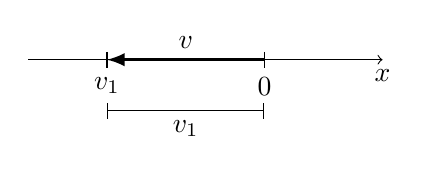
\begin{tikzpicture}[
	point/.style={circle,draw,very thin,fill,inner sep=0pt,minimum size=4pt},
	vector/.style={-latex},
]
	\coordinate (o) at (0,0);
	\coordinate (v) at (-2,0);
	\draw[->] (-3,0) to (1.5,0) node[below] {$x$};
	\draw[thin] ([shift={(0,0.1)}]o) to ([shift={(0,-0.1)}]o) node[below] {$0$};
	\draw[thin] ([shift={(0,0.1)}]v) to ([shift={(0,-0.1)}]v) node[below] {$v_1$};
	\draw[vector,very thick] (o) to node[above] {$\uvec{v}$} (v);
	\draw[|-|] ([shift={(0,-0.65)}]o) to node[below] {$\abs{v_1}$} ([shift={(0,-0.65)}]v);
\end{tikzpicture}
